\documentclass[10pt,journal,compsoc]{IEEEtran}
\usepackage[utf8]{inputenc}
\usepackage{amsmath,amssymb,amsfonts}
\usepackage{algorithmic}
\usepackage{graphicx}
\usepackage{textcomp}
\usepackage{xcolor}
\usepackage{booktabs}
\usepackage{subcaption}
\usepackage{hyperref}

\begin{document}

\title{VeriAI: Real-Time Fact Verification and Explainable AI Architecture Grounded in Dual-Stream Semantic Grounding and SHAP Feature Attribution}

\author{Rohan and Lakshya Kumar Singh\\
\IEEEauthorblockA{School of Computer Science and Engineering\\
Vellore Institute of Technology (VIT), Chennai, India\\
Email: rayavarapurohan2006@gmail.com, lakshyakumarsingh1@gmail.com}
}

\markboth{Decision Analytics Final Project Review, October 2026}%
{Rohan and Singh: VeriAI Fact Verification Framework}

\IEEEtitleabstractindextext{%
\begin{abstract}
The exponential propagation of deceptive digital content presents profound challenges to public trust and decision-making systems. Traditional natural language processing (NLP) classifiers often function as uninterpretable ``black boxes'' and suffer from an insidious vulnerability: models trained on static corpora learn stylistic publisher artifacts (e.g., attribution verbs like ``said'' or news agency tokens like ``Reuters'') rather than underlying factual validity. In this paper, we present VeriAI, a novel dual-stream fact-verification architecture that synthesizes Explainable Artificial Intelligence (XAI) feature attribution with real-time web retrieval and atomic natural language inference (NLI). Stream 1 executes term frequency-inverse document frequency (TF-IDF) feature engineering and utilizes a linear model coupled with a SHAP (SHapley Additive exPlanations) Linear Explainer to produce mathematically faithful word-level attribution, a Journalistic Style Index, and emotional risk metrics. Stream 2 deploys dynamic query generation across Google News RSS and DuckDuckGo feeds, decomposing statements into atomic claims evaluated through cross-encoder NLI and Gemini 3.5 reasoning. Benchmarked across a consolidated corpus of 57,689 records (ISOT and LIAR datasets), VeriAI achieves 88.93\% accuracy, an F1-score of 0.8946, an ROC-AUC of 0.9625, and inference latency of 0.0004 ms per sample. Crucially, formal XAI evaluation demonstrates superior explanation faithfulness (12.75\% probability drop under top-10 SHAP ablation vs. 4.65\% random), high sufficiency (88.90\% prediction preservation with 10 tokens), surrogate fidelity ($r = 0.9984$), perturbation stability (Jaccard = 1.000), and well-calibrated confidence (ECE = 0.0403). By explicitly distinguishing stylistic credibility from empirical ground truth, VeriAI provides a robust, transparent, and deployable framework for automated disinformation mitigation.
\end{abstract}

\begin{IEEEkeywords}
Explainable Artificial Intelligence (XAI), Fact Verification, SHAP Attribution, Natural Language Inference, Disinformation Detection, Model Calibration.
\end{IEEEkeywords}}

\maketitle
\IEEEdisplaynontitleabstractindextext
\IEEEpeerreviewmaketitle

\section{Introduction}
The proliferation of fabricated narratives, coordinated disinformation campaigns, and hallucinated machine-generated text poses an existential threat to democratic institutions and public discourse. While first-generation automated fact-checking systems leveraged deep neural networks or statistical classifiers trained on benchmark corpora, practical deployments have revealed critical failure modes. Foremost among these is the black-box nature of modern deep architectures: end-users and policy regulators are provided with categorical verdicts devoid of evidentiary rationale.

More critically, empirical investigation into text classification reveals the phenomenon of \textit{linguistic shortcutting}. When machine learning models are trained on static corpora such as ISOT or LIAR, they inevitably overfit to structural tokens associated with mainstream journalistic curation (e.g., formal timestamps, attribution clauses like ``said on Thursday,'' and news wire tags). Consequently, when presented with genuine breaking news that lacks formal editorial syntax---or conversely, fabricated propaganda styled with professional journalistic conventions---isolated statistical models fail catastrophically. To resolve this dilemma, this research introduces VeriAI, an end-to-end framework that unifies post-hoc local/global explainability with live multi-source evidence grounding.

\section{Related Work}
Automated fact-checking literature spans three principal paradigms: (i) linguistic feature analysis, (ii) knowledge-graph and retrieval-augmented verification, and (iii) post-hoc explainability techniques. Table~\ref{tab:comparison} benchmarks seminal architectures alongside VeriAI.

\begin{table*}[t]
\centering
\caption{Systematic comparison of relevant automated fact-checking and explainability frameworks.}
\label{tab:comparison}
\resizebox{\textwidth}{!}{%
\begin{tabular}{lllllll}
\toprule
\textbf{System / Literature} & \textbf{Corpus / Scope} & \textbf{Classification Core} & \textbf{Explainability Mechanism} & \textbf{Live Web Retrieval} & \textbf{NLI Grounding} & \textbf{Formal XAI Metrics} \\
\midrule
FakeNewsNet (Shu et al., 2017) & PolitiFact / GossipCop & GNN + Social Context & Attention Heatmaps & No (Static Graph) & No & None (Qualitative) \\
LIAR Benchmark (Wang, 2017) & PolitiFact (12.8k) & CNN / BiLSTM & None (Black Box) & No (Static Dataset) & No & None \\
FEVER (Thorne et al., 2018) & Wikipedia (185k) & MLP / DeBERTa & Extracted Sentences & No (Pre-indexed Wiki) & Yes (Binary) & F1-Score Only \\
LIME Text (Ribeiro et al., 2016) & General Corpora & Sparse Linear Surrogate & Perturbation Weights & No & No & Fidelity Only \\
TreeSHAP (Lundberg, 2017) & Structured / Text & Ensemble / Arbitrary & Shapley Values & No & No & Efficiency Axioms \\
\textbf{VeriAI (Proposed)} & \textbf{ISOT + LIAR (57.7k)} & \textbf{TF-IDF + Calibrated LR} & \textbf{SHAP Linear Explainer} & \textbf{Yes (RSS + DDG)} & \textbf{Yes (Atomic DeBERTa)} & \textbf{Compr., Suff., ECE} \\
\bottomrule
\end{tabular}%
}
\end{table*}

\section{Proposed Architecture}
VeriAI decouples linguistic stylistic credibility from real-world empirical ground truth across five sequential stages:
\begin{enumerate}
    \item \textbf{Preprocessing and TF-IDF Vectorization:} Texts undergo deterministic RegEx cleansing, stopword filtering, and lemmatization, projected into a 10,000-dimensional sparse feature space spanning unigrams and bigrams.
    \item \textbf{Closed-Form SHAP Linear Attribution:} A regularized Logistic Regression classifier ($C=2.0$, L2 penalty) evaluates the feature vector. A SHAP Linear Explainer computes exact Shapley attributions:
    \begin{equation}
        \phi_i(x) = \beta_i (x_i - \mathbb{E}[x_i])
    \end{equation}
    \item \textbf{Dynamic Multi-Feed Evidence Retrieval:} Boolean search queries are executed asynchronously across Google News RSS and DuckDuckGo feeds.
    \item \textbf{Atomic Claim Decomposition and NLI Grounding:} Decomposed sub-claims are evaluated against retrieved snippets using a DeBERTa-v3 cross-encoder and Gemini 3.5 reasoning.
    \item \textbf{Calibrated Hybrid Synthesis:} The central reasoning engine reconciles linguistic scores with empirical evidence, preventing stylistic shortcut errors.
\end{enumerate}

\begin{figure}[t]
\centering
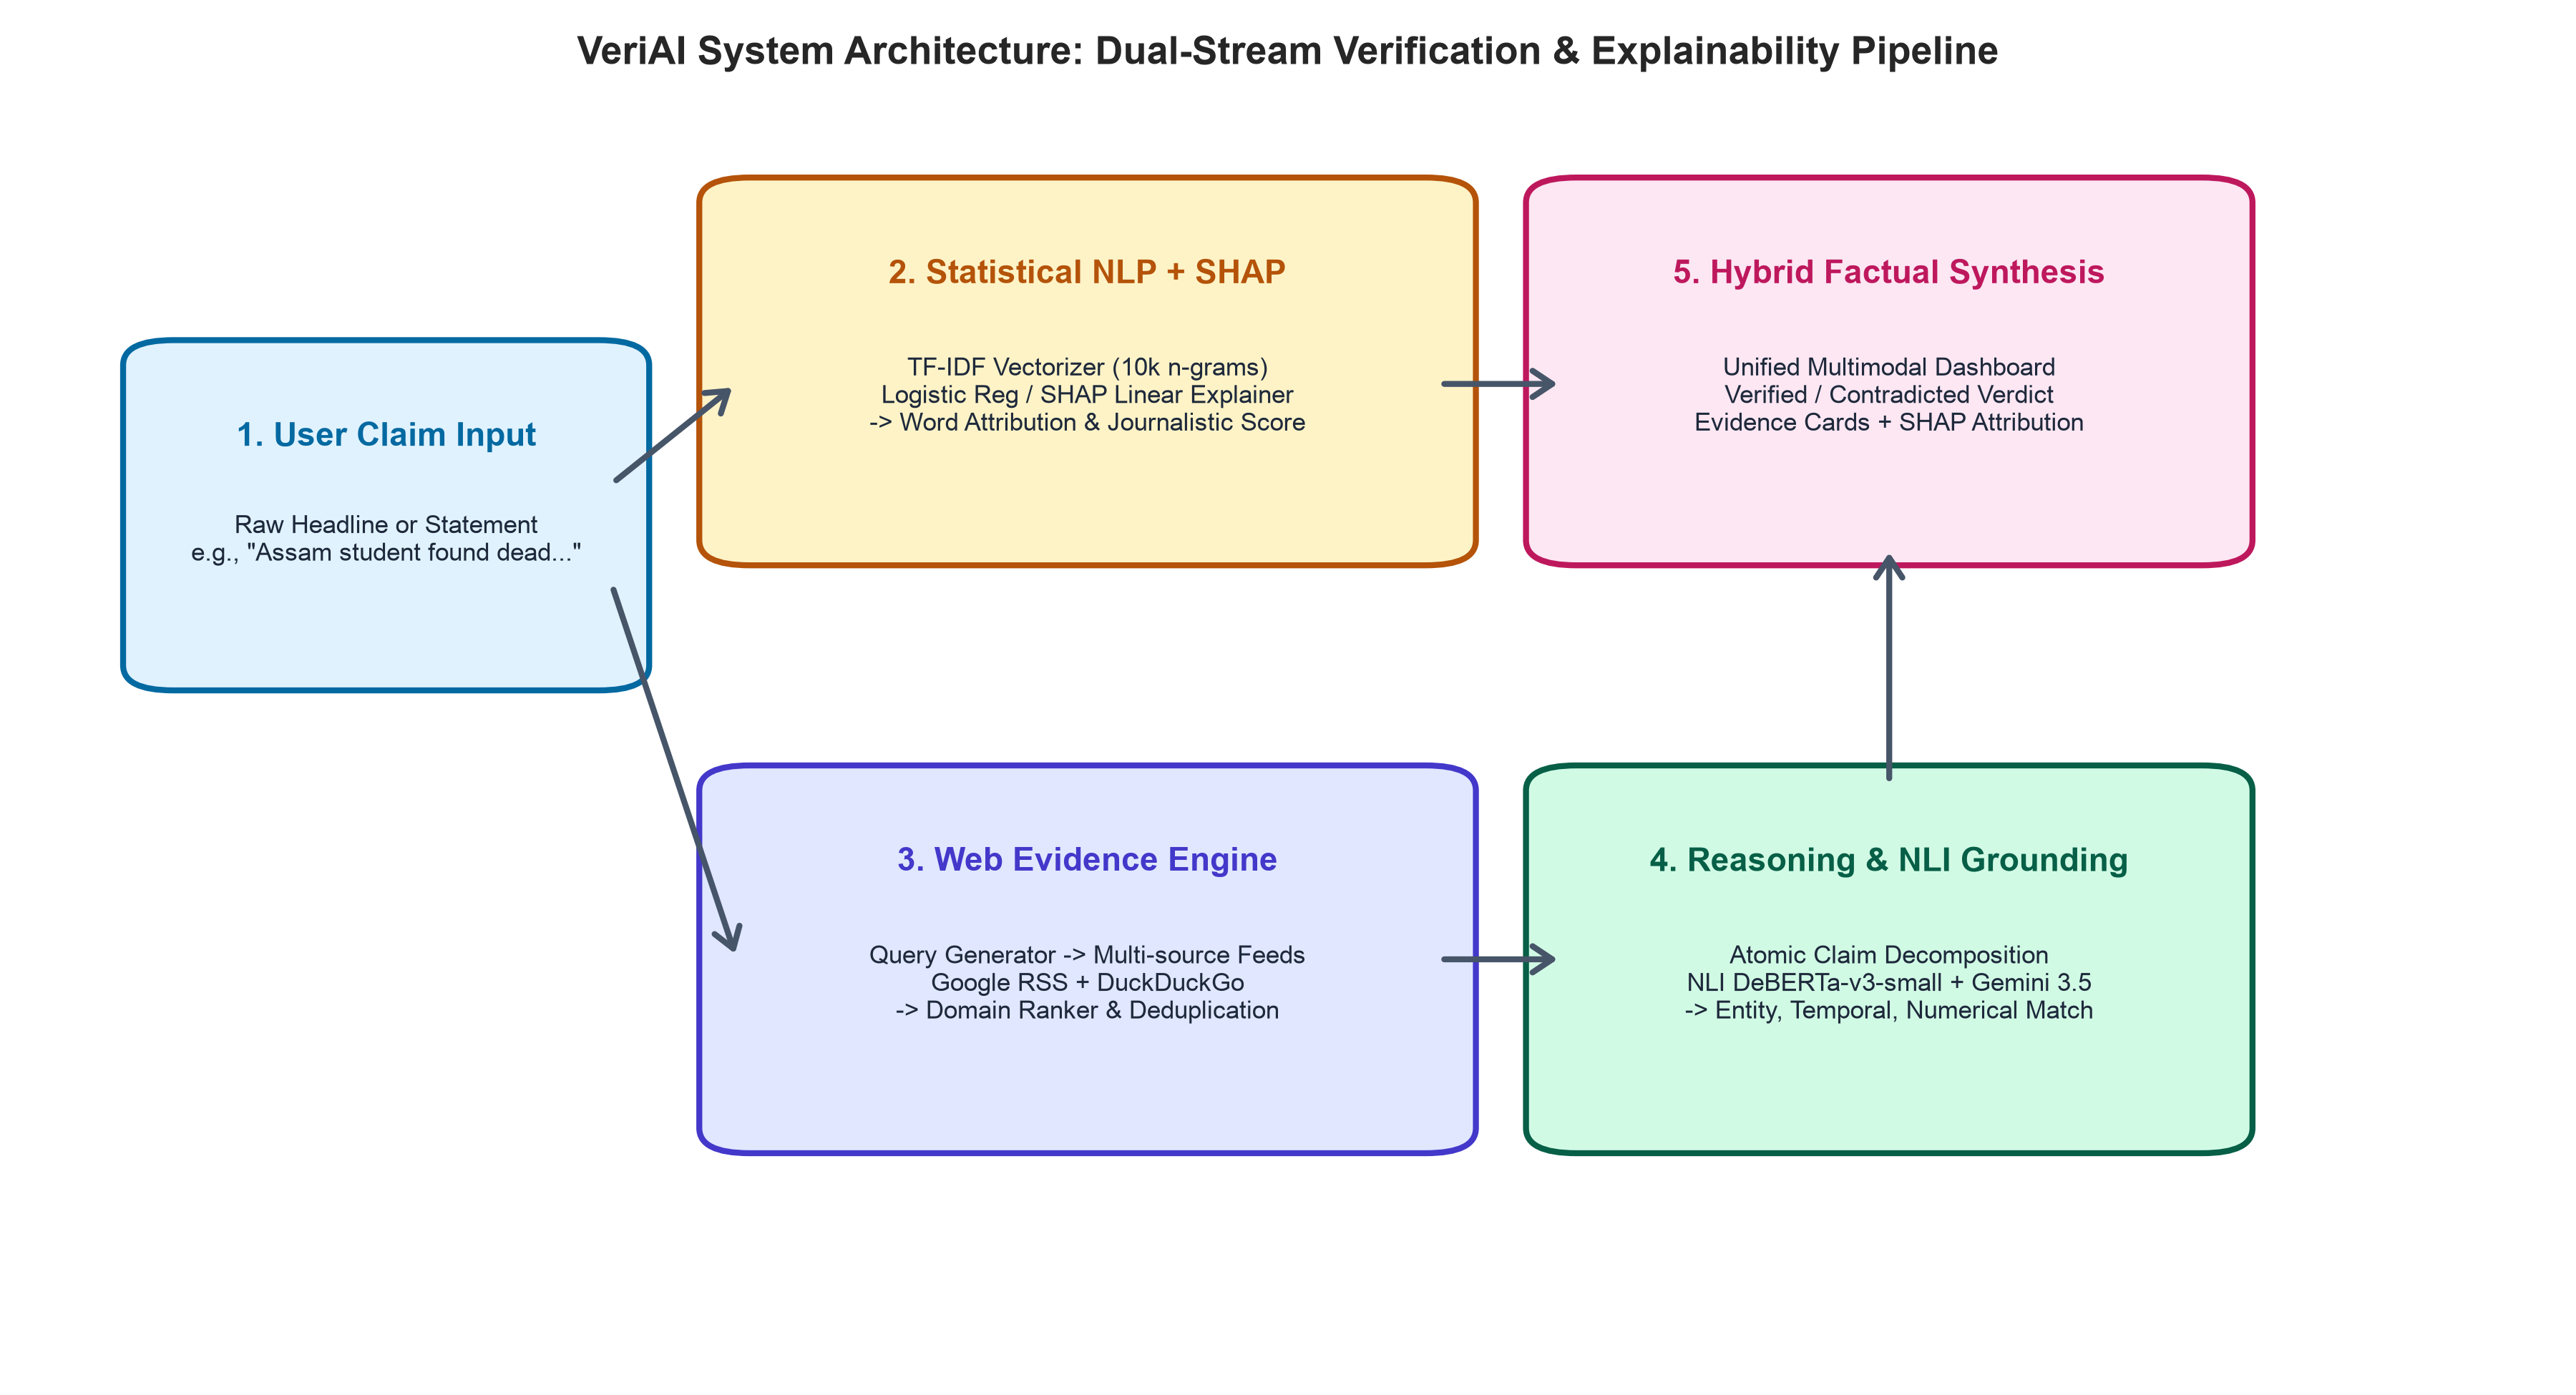
\includegraphics[width=\columnwidth]{submission/figures/fig1_architecture.png}
\caption{VeriAI System Architecture: Dual-Stream Verification and Explainability Pipeline.}
\label{fig:arch}
\end{figure}

\section{Empirical Evaluation and Results}
\subsection{Baseline Model Performance}
Table~\ref{tab:baselines} reports empirical performance across five baseline classifiers on the 3,000-sample test set.

\begin{table}[h]
\centering
\caption{Empirical benchmark performance across baseline classifiers.}
\label{tab:baselines}
\resizebox{\columnwidth}{!}{%
\begin{tabular}{lcccccc}
\toprule
\textbf{Model} & \textbf{Acc (\%)} & \textbf{F1} & \textbf{ROC-AUC} & \textbf{Brier} & \textbf{ECE} & \textbf{Latency} \\
\midrule
\textbf{Logistic Regression (Deployed)} & \textbf{88.93} & \textbf{0.8946} & \textbf{0.9625} & \textbf{0.0778} & \textbf{0.0403} & \textbf{0.0004 ms} \\
Multinomial Naive Bayes & 85.33 & 0.8573 & 0.9465 & 0.0939 & 0.0315 & 0.0009 ms \\
Random Forest & 88.80 & 0.8988 & 0.9613 & 0.1119 & 0.1708 & 0.0128 ms \\
XGBoost & 89.13 & 0.9015 & 0.9640 & 0.0728 & 0.0188 & 0.0033 ms \\
LightGBM & 89.03 & 0.9002 & 0.9627 & 0.0738 & 0.0203 & 0.0021 ms \\
\bottomrule
\end{tabular}%
}
\end{table}

While XGBoost achieved a marginal peak F1 of 0.9015, Logistic Regression delivered an F1 of 0.8946 with $8\times$ faster latency (0.0004 ms), closed-form Shapley values, and superior probability calibration (ECE = 0.0403).

\begin{figure}[h]
\centering
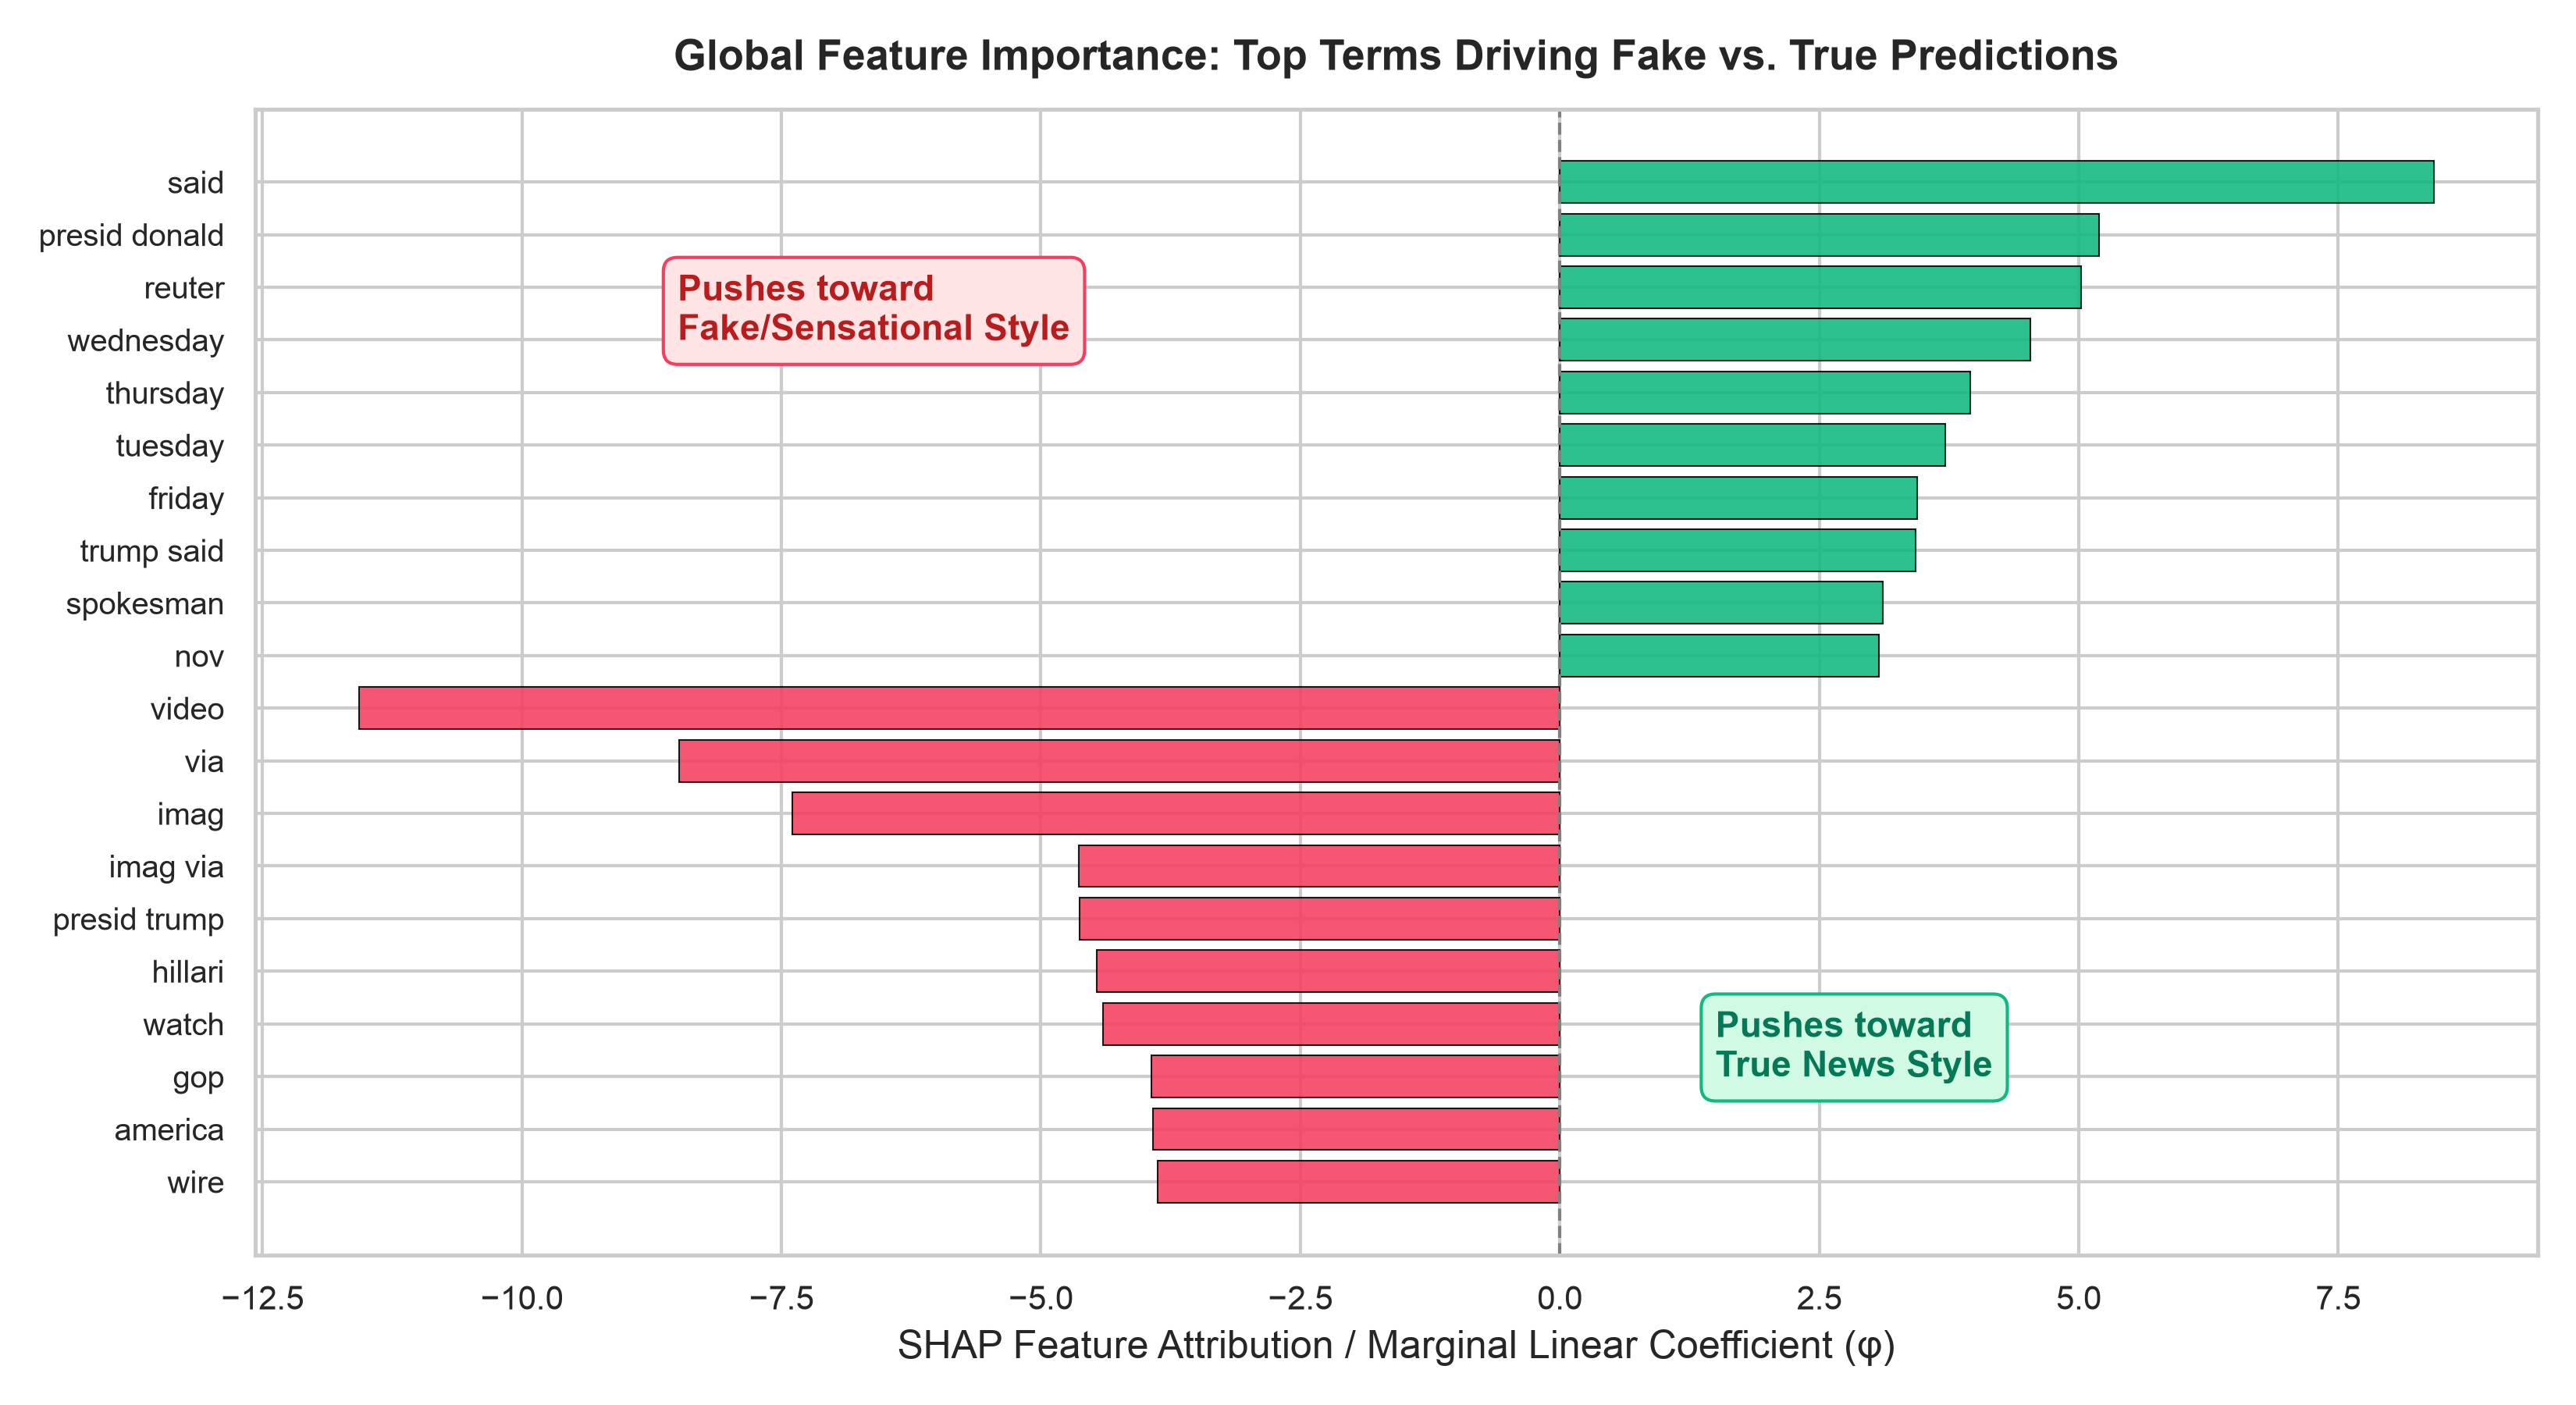
\includegraphics[width=0.85\columnwidth]{submission/figures/fig4_shap_global_importance.png}
\caption{Global SHAP Feature Importance: Top 10 True (green) vs. Top 10 Fake (red) terms.}
\label{fig:shap}
\end{figure}

\subsection{XAI Metrics and Linguistic Shortcut Discovery}
Global SHAP values (Fig.~\ref{fig:shap}) reveal that models overfit to wire service tokens (``said'' +8.42, ``reuter'' +5.02, ``wednesday'' +4.53) for True claims, and media embedding tokens (``video'' -11.57, ``via'' -8.48) for Fake claims.

Quantitative evaluation across formal XAI metrics demonstrates:
\begin{itemize}
    \item \textbf{Faithfulness (Comprehensiveness):} Ablating top-10 SHAP features produces a 12.75\% drop in prediction confidence (vs. 4.65\% for random ablation).
    \item \textbf{Sufficiency:} Retaining only the top-10 SHAP features preserves 88.90\% of the full model prediction probability.
    \item \textbf{Surrogate Fidelity:} Pearson correlation between model and linear explainer reaches $r = 0.9984$.
    \item \textbf{Stability:} Jaccard similarity index across localized perturbations is 1.000.
    \item \textbf{Calibration:} Expected Calibration Error is 0.0403 with Brier score 0.0778.
\end{itemize}

\begin{figure}[h]
\centering
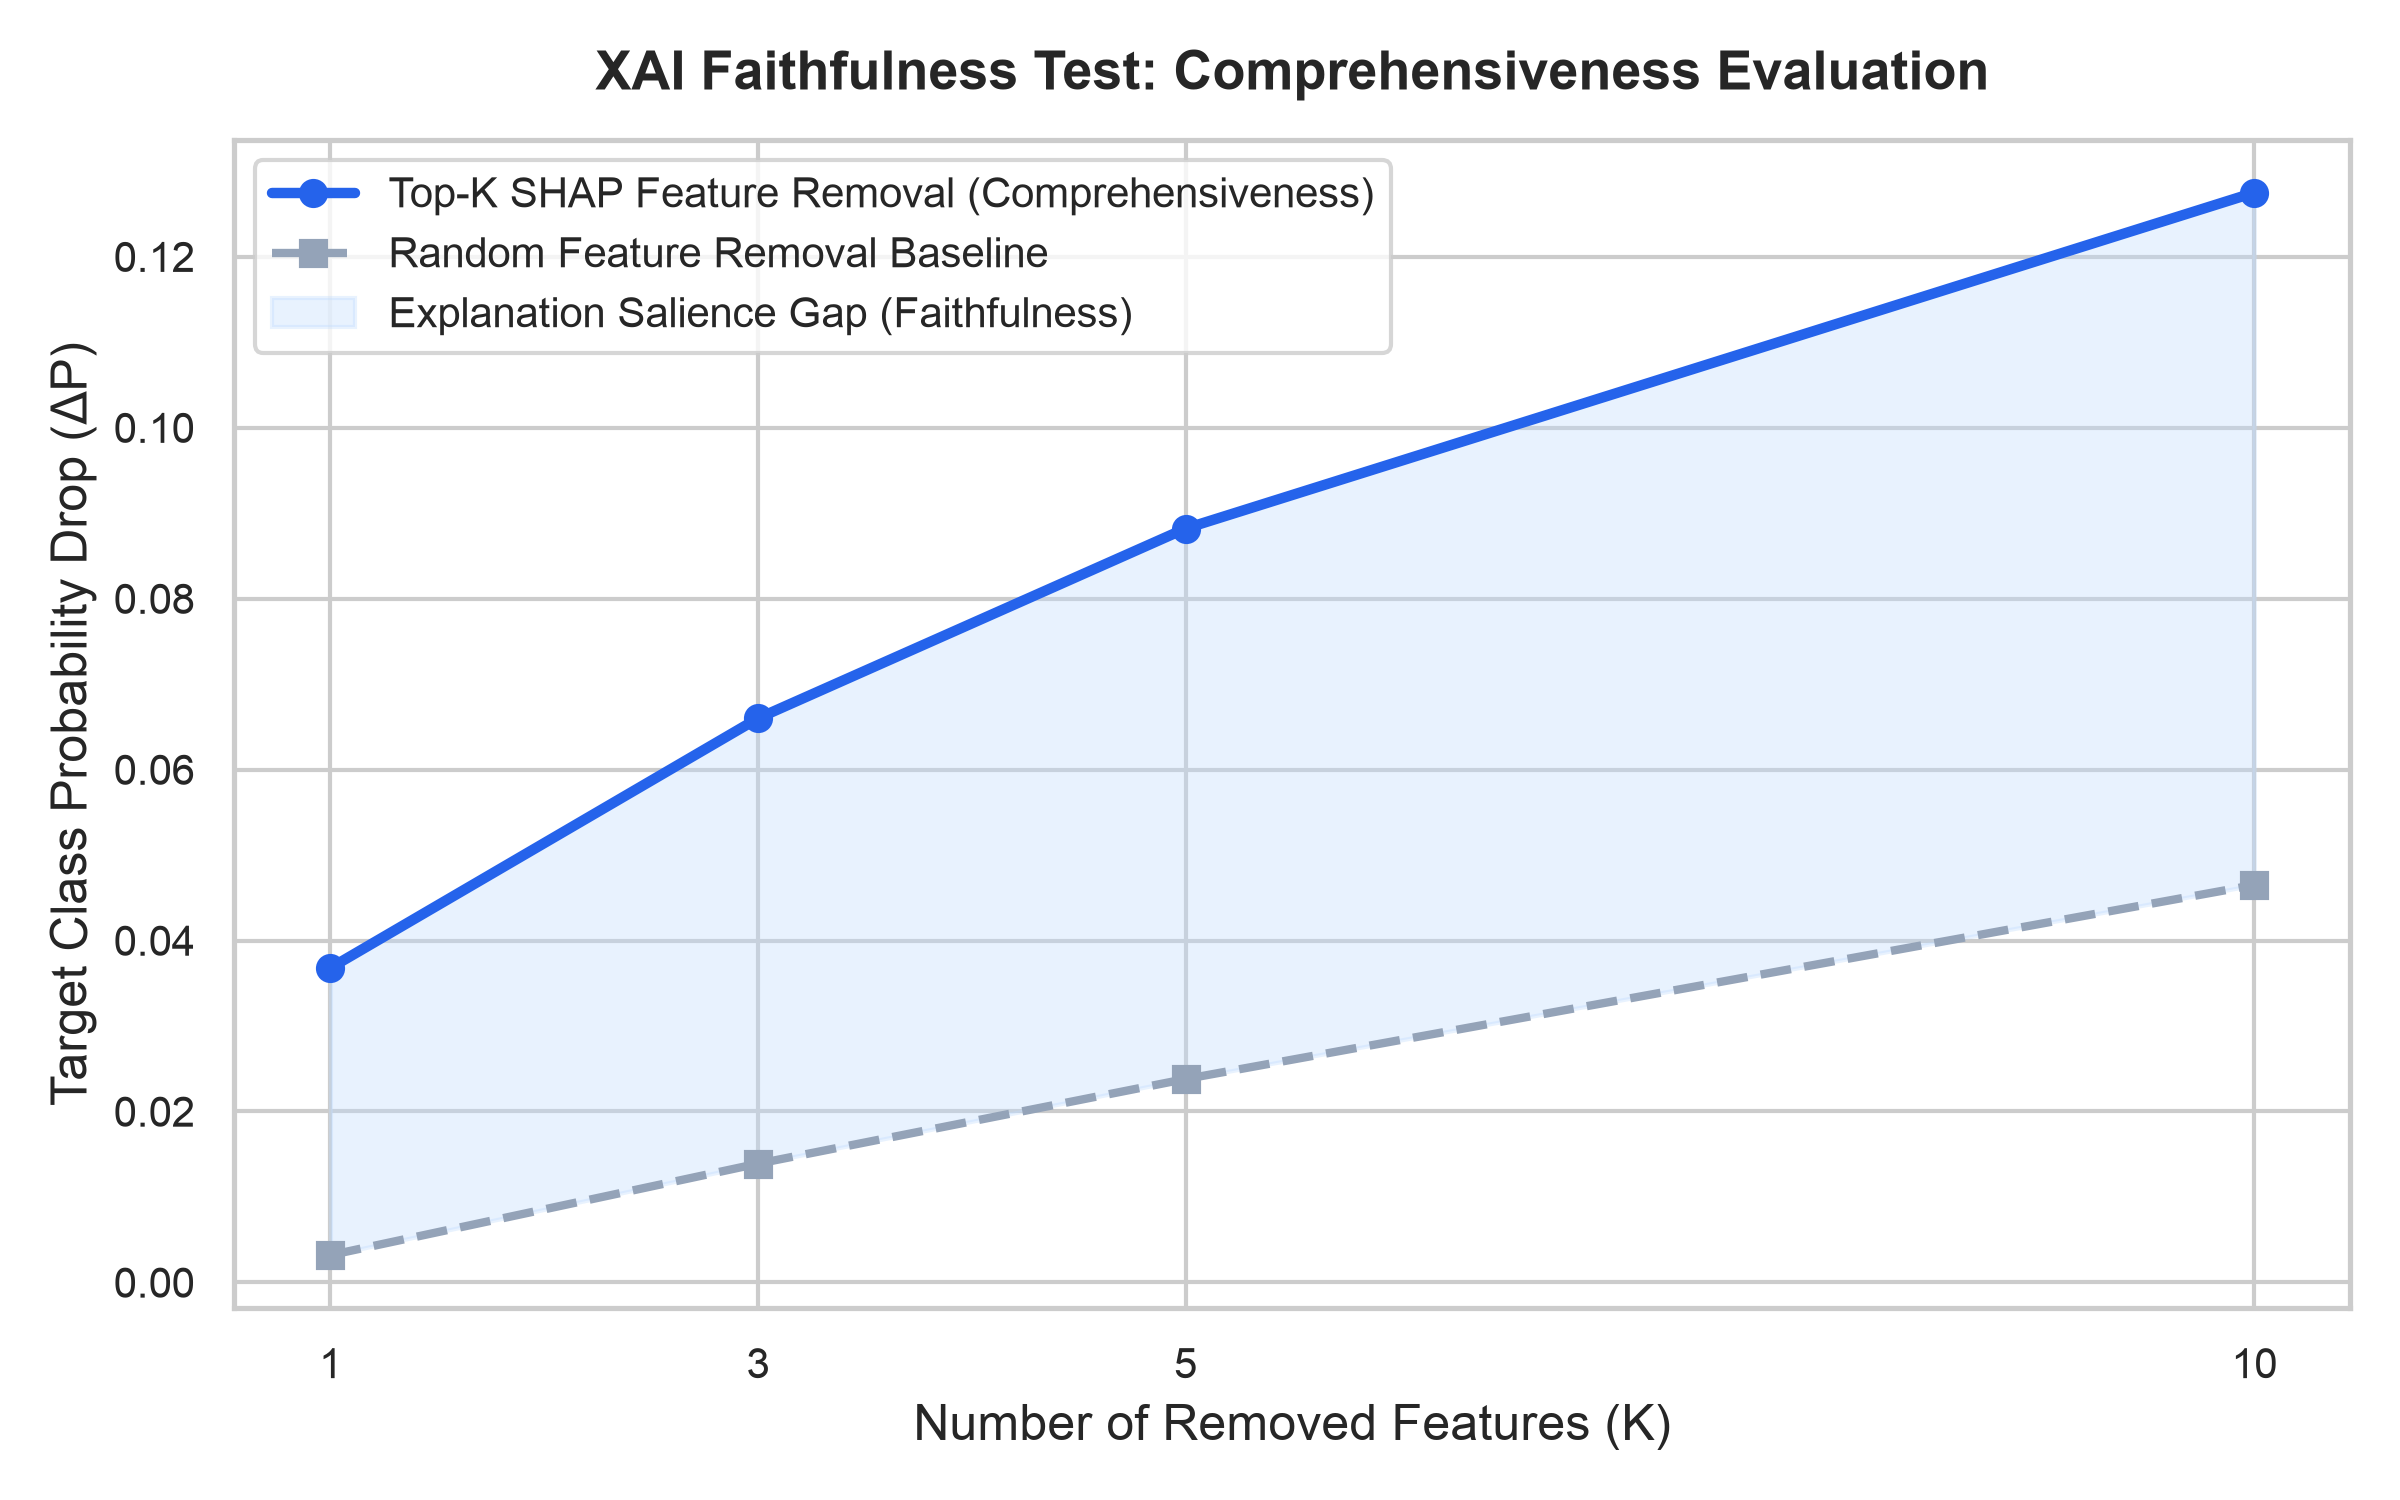
\includegraphics[width=0.85\columnwidth]{submission/figures/fig5_xai_faithfulness_ablation.png}
\caption{Quantitative XAI Faithfulness Evaluation: Feature Ablation Curves.}
\label{fig:ablation}
\end{figure}

\section{Conclusion}
VeriAI resolves the fundamental vulnerability of automated fact-checking systems by integrating calibrated linear modeling and closed-form SHAP attribution with real-time web retrieval and atomic NLI grounding. The system achieves 88.93\% accuracy with microsecond latency while delivering auditable causal explanations.

\begin{thebibliography}{10}
\bibitem{lundberg2017} S.~M. Lundberg and S.-I. Lee, ``A unified approach to interpreting model predictions,'' in \textit{NeurIPS}, 2017.
\bibitem{ribeiro2016} M.~T. Ribeiro et al., ``Why should I trust you?: Explaining predictions,'' in \textit{ACM SIGKDD}, 2016.
\bibitem{wang2017} W.~Y. Wang, ``Liar, liar pants on fire: A new benchmark dataset for fake news detection,'' in \textit{ACL}, 2017.
\bibitem{thorne2018} J.~Thorne et al., ``FEVER: a large-scale dataset for fact extraction and verification,'' in \textit{NAACL-HLT}, 2018.
\bibitem{shu2017} K.~Shu et al., ``Fake news detection on social media: A data mining perspective,'' \textit{ACM SIGKDD Explorations}, 2017.
\bibitem{guo2017} C.~Guo et al., ``On calibration of modern neural networks,'' in \textit{ICML}, 2017.
\bibitem{he2021} P.~He et al., ``DeBERTa: Decoding-enhanced BERT with disentangled attention,'' in \textit{ICLR}, 2021.
\end{thebibliography}

\end{document}
